\chapter{La radioterapia adattiva. Implementazione iniziale e sviluppi futuri}
\minitoc
\textsf{}

\section{Origini e razionale della radioterapia adattiva}
Per radioterapia adattiva o \textit{adaptive radiation therapy} si intende una tecnica di erogazione della dose che si `adatta' ai possibili cambiamenti che si verificano durante il trattamento, rispetto alla situazione iniziale di pianificazione. I cambiamenti che si possono verificare durante un trattamento radiante possono essere di varia natura e riguardare sia l'interno del paziente (progressione/regressione del target, dimagrimento, diverso stato di riempimento degli organi cavi), sia il suo  posizionamento sul lettino di trattamento (incertezza di setup). 

Il metodo tradizionale di affrontare il problema dei cambiamenti rispetto alla situazione di pianificazione è esposto nei report della \textit{International Commission of Radiological Units} (ICRU) no.50 e no.62, ripreso anche nel recente report no.83 per le tecniche ad intensità modulata \cite{ICRU2010}. Esso consiste nell'espandere i target di un certo margine di sicurezza in modo da assicurare la loro corretta irradiazione anche in presenza delle succitate incertezze.
\begin{figure}
\centering
a)\includegraphics[width=.25\textwidth]{./cap3/ptv.png}
b) \includegraphics[width=.64\textwidth]{./cap3/adapt0.png}
\caption{(a) definizioni ICRU dei volumi coinvolti nella pianificazione del trattamento radioterapico. (b) Processo standard di pianificazione ed erogazione del piano del trattamento.}
\label{fig:adapt0}
\end{figure}

Nella Fig.\ref{fig:adapt0} sono riportate le definizioni dei volumi coinvolti nella pianificazione del trattamento radioterapico assieme ad uno schema del processo standard di pianificazione ed erogazione del piano del trattamento.\\
Il meccanismo che ha portato alla definizione dei singoli volumi procede in vari step:
\begin{description}
\item[Gross Target Volume (GTV):] questo volume identifica il tumore a livello macroscopico (rivelabile attraverso strumenti ottici, imaging radiologico, esame obiettivo clinico,\ldots).

\item[Clinical Target Volume (CTV):] volume che comprende il GTV ed un margine attorno ad esso in cui vi è alta probabilità di presenza di malattia che ancora non si manifesta clinicamente (sub-clinica).

\item[Internal Target Volume (ITV):] volume che aggiunge al CTV un margine (detto \textit{internal margin o IM}) che serve a comprendere il possibile movimento del target per cause interne al paziente (e.g. respiro, stato di riempimento degli organi adiacenti, battito cardiaco\ldots).

\item[Planning Target Volume (PTV):] volume che aggiunge all'ITV un margine per comprendere l'incertezza dovuta al posizionamento del paziente rispetto alla posizione di pianificazione (\textit{setup margin o SM}).

\item[Treated Volume:] volume che riceve una dose maggiore del 98\% della dose di prescrizione.

\end{description}

Il metodo per calcolare i margini necessari alla definizione del PTV si basa su uno studio statistico in cui si effettua un analisi dei possibili errori di posizionamento del target rispetto alla posizione pianificata, distinguendoli in errori sistematici ed errori random. Una delle formule più note è dovuta a Marcel Van Herk \cite{ICRU62}:
\begin{equation}
PTV_{margin} = 2.5\Sigma + 0.7\sigma
\end{equation}
dove $\Sigma$ rappresenta l'errore sistematico ossia quell'errore che si ripete per tutto il ciclo di trattamento (es. paziente dimagrito rispetto alla pianficazione) mentre $\sigma$ è l'errore random (es. movimento d'organo).

In un approccio non adattivo i margini da dare al CTV per arrivare al PTV si trovano effettuando uno studio di coorte per un fissato sito di irradiazione. In questo studio si valutano gli errori sistematici e random su una popolazione di pazienti e si applica la formula di Van Herk secondo le direttive ICRU \cite{ICRU62}. La pianificazione viene quindi effettuata stabilendo delle condizioni di irradiazione del planning target volume (PTV)  che vengono ripetute per tutto il ciclo di trattamento (Fig.\ref{fig:adapt0}b).\\
Questo tipo di approccio può tuttavia non essere ottimale per lo specifico paziente come indicato schematicamente nella Fig.\ref{fig:margins}. In un approccio di \textit{adaptive radiotherapy} è invece possibile studiare il singolo caso ed adattare il trattamento allo specifico paziente.
\begin{figure}
\centering
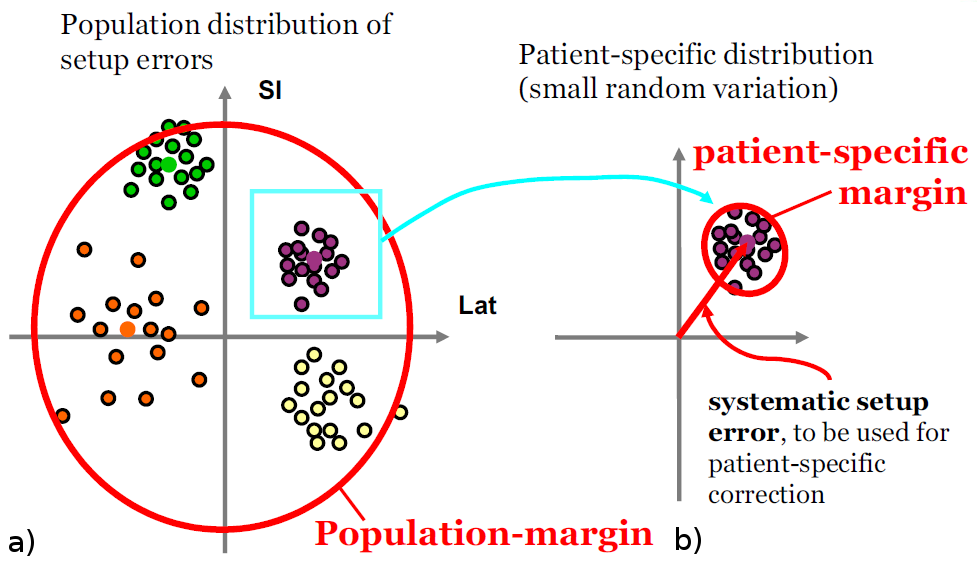
\includegraphics[width=.8\textwidth]{./cap3/margins.png}
\caption{La formula di Van Herk per ottenere il PTV utilizzando uno studio di coorte (a) da luogo a margini che possono essere sovrabbondanti per il singolo paziente (b).}
\label{fig:margins}
\end{figure}

Il termine \textit{adaptive radiotherapy} è stato introdotto per la prima volta  da Yan et al.\cite{Yan1996}. In questo lavoro veniva per la prima volta proposto un adattamento del piano di cura a seguito di rilevazioni effettuate nelle prime cinque sedute di trattamento con un dispositivo in grado di `fotografare' la posizione del paziente e di confrontarla rispetto alla posizione di pianificazione. Il dispositivo in oggetto è denominato \textit{portal imager} e consiste in un pannello elettronico montato sul LINAC che è in grado di generare un'immagine utilizzando raggi di energia dell'ordine dei MeV allo stesso modo in cui vengono generate le radiografie classiche con i raggi di energia dell'ordine del keV. A seguito di queste rilevazioni Yan proponeva di stimare l'errore sistematico paziente-specifico calcolando la media delle deviazioni tra posizione pianificata e posizione di trattamento rilevate nelle prime cinque sedute e di adattare il piano spostando il centro di irradiazione di questa quantità.

\begin{figure}[!t]
\centering
a)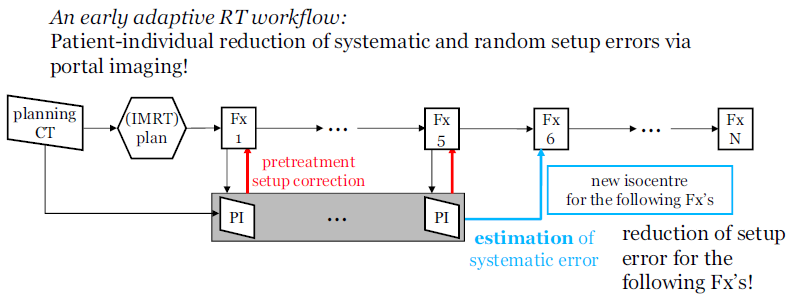
\includegraphics[width=.95\textwidth]{./cap3/adapt1.png}
b)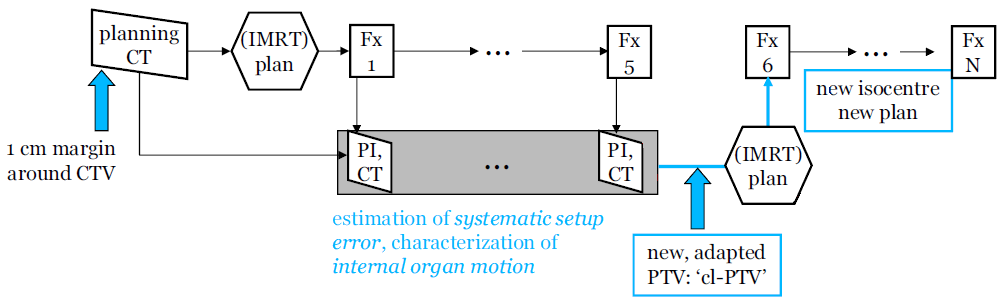
\includegraphics[width=.95\textwidth]{./cap3/adapt2.png}
\caption{(a) approccio di adaptive radiotherapy in cui viene unicamente modificato l'isocentro del piano a seguito di rilevazioni dell'errore di posizionamento del paziente tramite portal-imager (PI). (b) approccio di adaptive radiotherapy in cui alla modificazione dell'isocentro si aggiunge la modificazione dei margini attorno al CTV in base a rilevazioni di tomografia computerizzata (CT); in questo caso il piano di trattamento si adatta al nuovo PTV \textit{confidence-limit PTV o cl-PTV} stimato dopo le cinque sedute di controllo.}
\label{fig:adaptYAN}
\end{figure}

Pochi anni dopo sempre Yan et al.\cite{Yan2000} pubblicano un altro studio in cui aggiungono alla rilevazione tramite portal-imager anche un rilevazione di tomografia computerizzata del paziente per le prime cinque sedute in modo da osservare il problema del movimento d'organo oltre all'errore di setup. Questo permise agli autori di definire un PTV paziente-specifico che veniva calcolato con la procedura seguente:
\begin{itemize}
\item Si delinea il CTV sui cinque studi CT acquisite in sede delle prime cinque frazioni di trattamento.
\item Si uniscono i contorni dei cinque CTV con il CTV di pianficazione a costituire il cosiddetto \textit{CTV-hull}.
\item Si espande il \textit{CTV-hull} del margine corrispondente all'errore sistematico misurato tramite le cinque rilevazioni tramite portal-imager per formare il \textit{confidence-limit PTV o cl-PTV}. 
\end{itemize}
Entrambi gli approcci adaptive presentati in questa sezione sono raffigurati schematicamente nella Fig.\ref{fig:adaptYAN}.

\`E stato dimostrato che la riduzione del PTV e la conseguente ripianficazione possibile grazie all'applicazione di queste tecniche di adaptive radiotherapy ha portato ad un decremento significativo delle tossicità per gli organi sani, preservando il controllo della malattia \cite{Park2012}. Questo dato è facilmente comprensibile con il paradigma dell'arancia di Verellen \cite{Verellen2007} illustrato in Fig.\ref{fig:verellen}. In pratica, il volume occupato dalla buccia di un'arancia è comparabile con il volume dell'arancia stessa. Tradotto, la riduzione anche di pochi millimetri del PTV può comportare una riduzione del volume da irradiare considerevole che porta ad un maggior risparmio dei tessuti sani.
\begin{figure}[!t]
\centering
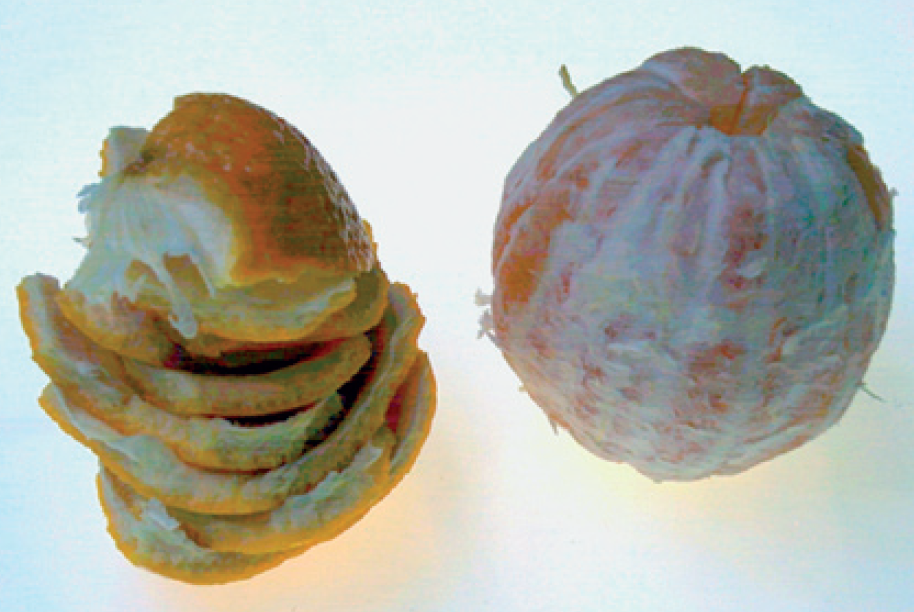
\includegraphics[width=.6\textwidth]{./cap3/Verellen.png}
\caption{Il paradigma dell'arancia di Verellen \cite{Verellen2007} per illustrare l'importanza della riduzione dei margini in radioterapia.}
\label{fig:verellen}
\end{figure}



\section{Il concetto attuale di \textit{adaptive-radiotherapy} implementato in RayStation}
Il concetto di radioterapia adattiva ha subito negli anni vari aggiornamenti e revisioni ma solo negli ultimi anni è divenuto oggetto di grande interesse. Ciò è dovuto principalmente all'avvento  delle tecniche di imaging per il controllo volumetrico del posizionamento del paziente installate sui moderni LINAC. La tecnica più diffusa implementata nei moderni LINAC è denominata \textit{cone-beam-computed-tomography o CBCT}. Essa consiste in un sistema capace di ricostruire immagini tomografiche del paziente utilizzando un fascio conico di raggi X e di confrontarle con lo studio CT di pianificazione.

\begin{figure}[!t]
\centering
\centerline{
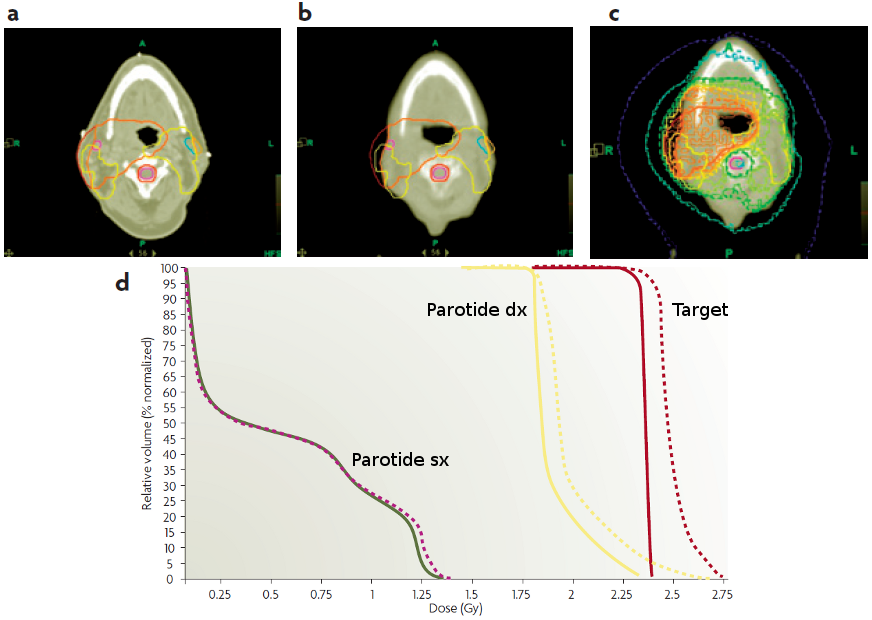
\includegraphics[width=1.2\textwidth]{./cap3/HN_DVH.png}}
\caption{(a) scansione CT del distretto testa-collo di un paziente con delineato in rosso il target e negli altri colori gli organi a rischio. (b) scansione CBCT di controllo a 2.5 settimane con evidente riduzione di volume del target. (c-d) confronto delle distribuzioni di dose di pianificazione (linea continua) e di valutazione (linea tratteggiata). L'istogramma (d) è detto \textit{istogramma dose-volume o DVH} e rappresenta quantitativamente come la distribuzione di dose copre i volumi delineati nello studio CT. \`E da notare come il cambiamento del paziente comporti una variazione della distribuzione di dose agli organi e al target.}
\label{fig:HN_DVH}
\end{figure}

 Nella Fig.\ref{fig:HN_DVH} è illustrato un tipico esempio di irradiazione del distretto testa-collo di largo interesse per la radioterapia adattiva per i grossi cambiamenti che avvengono in itinere nell'anatomia del paziente. A causa dei rapidi gradienti di dose realizzati con le tecniche ad intensità modulata, piccoli cambiamenti di anatomia del paziente possono avere un largo impatto sulla distribuzione di dose finale sia per il target che per gli organi a rischio (Fig.\ref{fig:HN_DVH}d). \\
 
Il TPS RayStation affronta il problema della radioterapia adattiva offrendo una soluzione `all-in-one' che si articola in cinque principali step:
\begin{itemize}
\item[\textbf{a)}] \textbf{Acquisizione degli studi CBCT:} le CBCT acquisite dal sistema di imaging montato sul LINAC vengono spedite al TPS.
\item[\textbf{b)}] \textbf{Deformazione elastica:} viene effettuata una registrazione elastica tra la CT di pianificazione e le CBCT. Questa operazione consiste nel trovare il campo di deformazione geometrico che, se applicato alla CBCT di controllo,   trasforma quest'ultima nella CT di pianificazione. La trasformazione in oggetto è unicamente geometrica: vengono solo variate le coordinate dei pixel ma non il loro valore in scala di grigi.
\item[\textbf{c)}] \textbf{Calcolo della dose in CBCT:} il piano di trattamento viene trasferito alle CBCT e ricalcolato in modo da ottenere la distribuzione di dose relativa alle specifiche frazioni. 
\item[\textbf{d)}] \textbf{Deformazione delle dosi:} sulla base della registrazione deformabile geometrica viene deformata la distribuzione di dose calcolata in CBCT e riportata sulla CT di pianificazione. In questo modo si possono confrontare le distribuzioni di dose pianificata ed effettivamente erogata sulla CT di pianificazione.
\item[\textbf{e)}] \textbf{Adattamento del piano:} sulla base delle differenze tra le distribuzioni di dose pianificata ed erogata si decide o meno di effettuare una ripianificazione del trattamento.
\end{itemize}

Tutti questi passaggi (a parte il primo) presentano delle criticità che al giorno d'oggi non sono del tutto superate in maniera condivisa. In particolare, le questioni su cui vi è ancora un largo dibattito nella comunità scientifica possono essere riassunte nei punti seguenti:\\

\noindent\textbf{Deformazione elastica:}
\begin{itemize}
\item Quale accuratezza è raggiungibile?
\item Quale è il miglior modo di effettuare le deformazioni?
\end{itemize}
\textbf{Calcolo della dose in CBCT}
\begin{itemize}
\item Quanto è accurato il calcolo della dose in CBCT?
\end{itemize}
\textbf{Deformazione delle dosi:}
\begin{itemize}
\item Quanto è giusto deformare le dosi utilizzando la trasformazione geometrica?
\end{itemize}
\textbf{Adattamento del piano:}
\begin{itemize}
\item Sulla base di quale metrica si può decidere la ripianificazione?
\item Qual è il momento migliore per la ripianificazione?
\item Che livello di verifica pre-trattamento è richiesto per il piano adattato?
\end{itemize}

Come mostrato in un recente point/counterpoint pubblicato su \textit{Medical Physics} \cite{Schultheiss2012}, la comunità scientifica non è ancora giunta ad una risposta precisa ed esaustiva per le domande sopra elencate. Per questo motivo il commissioning del TPS dal punto di vista della radioterapia adattiva risulta tutt'ora in fase di ottimizzazione. In particolare, gli sforzi che si stanno compiendo in questo senso consistono nella partecipazione a due studi multicentrici nazionali orientati a chiarire gli aspetti più dibattuti ossia quelli riguardanti la deformazione elastica e l'adattamento del piano.

\section{Studio multicentrico per l'ottimizzazione del protocollo di deformazione elastica}
Il TPS RayStation implementa un algoritmo di deformazione elastica ibrido \cite{RaySearchLaboratories2014}. In particolare, il campo di deformazione viene trovato considerando la differenza tra i livelli di grigio tra lo studio di riferimento e lo studio target, assieme alla presenza di eventuali strutture geometriche che fungono da guida (ROI di controllo).

Ciò si realizza matematicamente minimizzando un funzionale cha ha la forma seguente:
\begin{equation}
\label{eq:def}
\begin{split}
F =& \alpha \cdot (1- Correlation\, Coefficient) + \\
   & + \beta \cdot Regularization\,Term + \\
   & + \gamma \cdot ROI\,Penalty\,Term
\end{split}
\end{equation}
dove il \textit{Correlation coefficient} è un termine del tipo coefficiente di correlazione di Pearson e misura la correlazione tra i livelli di grigio delle due immagini (è uguale a 1 per immagini identiche). Il termine di regolarizzazione (\textit{Regularization Term}) aumenta all'aumentare dell'intensità della deformazione e serve a penalizzare soluzioni improbabili dal punto di vista fisico. Infine il \textit{ROI Penalty Term} è un termine che diminuisce quanto più le ROI di controllo tra le due immagini sono sovrapposte.

Nella corrente implementazione dell'algoritmo di deformazione in RayStation (v.4.7) i termini peso $\alpha$, $\beta$ e $\gamma$, il coefficiente di correlazione ed il termine di regolarizzazione sono tutti fissati dalla ditta. Quello che viene lasciato all'operatore è la scelta delle ROI di controllo (ultimo termine della Eq.\eqref{eq:def}).

Il razionale dello studio multicentrico cui si è presi parte consiste nell'investigare l'accuratezza di vari algoritmi di registrazione deformabile disponibili commercialmente e di sviluppare le metodologie che portano alla migliore deformazione possibile. A questo proposito è stato riunito un gruppo di 13 istituzioni italiane (Gruppo YES - Your Elastic Solution) per un totale di 5 diverse soluzioni commerciali per la registrazione elastica, tra cui il TPS RayStation. Lo studio si articola in più fasi ed è tutt'ora in corso di svolgimento. Nell'ambito di questo lavoro di tesi discuteremo i risultati raggiunti nella fase riguardante i casi clinici.

Per la fase clinica dello studio YES sono stati reclutati 3 studi CT per i distretti pelvico, testa-collo e polmonare (Fig.\ref{fig:YES_sites}).
\begin{figure}
\centering
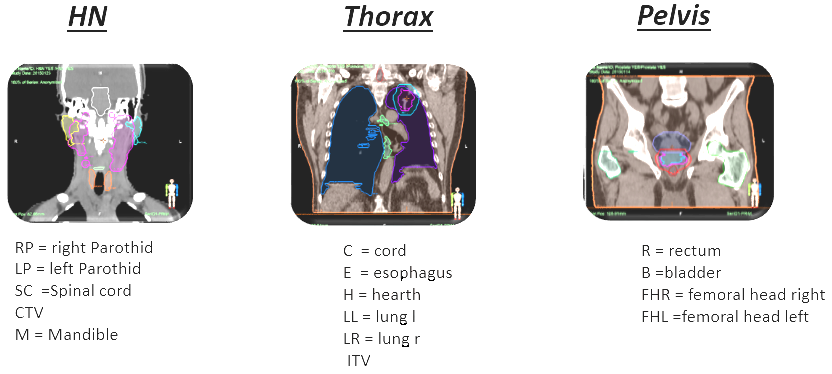
\includegraphics[width=\textwidth]{./cap3/YES_Sites.png}
\caption{Siti anatomici studiati nell'ambito del gruppo YES}
\label{fig:YES_sites}
\end{figure}
Per ogni distretto è stato creato un altro studio CT in cui è stata simulata tramite software (ImSimQA) una deformazione che tipicamente si realizza nella routine clinica:
\begin{itemize}
\item[\textbf{a)}] \textbf{Distretto pelvico:} riempimento vescicale minore rispetto alla CT di pianificazione ed aumento del volume rettale.
\item[\textbf{b)}] \textbf{Distretto testa-collo:} riduzione del volume linfonodale.
\item[\textbf{c)}] \textbf{Distretto polmonare:} riduzione di volume del tumore.
\end{itemize}
Ogni istituzione aveva il compito di ricavare in maniera inversa la deformazione simulata utilizzando gli strumenti in proprio possesso. Sulla base della deformazione ottenuta veniva richiesto di mappare delle regioni di interesse (ROI) dalla CT iniziale alla CT deformata. Le ROI mappate da ogni centro sono state poi confrontate con le ROI `gold' deformate secondo la deformazione introdotta via software, nota solo al centro coordinatore.\\
L'indicatore utilizzato per confrontare le ROI mappate dai centri con le ROI `gold' è l'indice di conformità di Jaccard:
\begin{equation}
CI(ROI_{A},ROI_{B}) = \frac{|ROI_{A} \cap ROI_{B}|}{|ROI_{A} \cup ROI_{B}|}
\end{equation}
Questo indice è uguale a 0 per ROI disgiunte mentre è uguale a 1 per ROI esattamente sovrapposte.
I risultati raggiunti a livello multicentrico sono riassunti principalmente nei seguenti punti:
\begin{itemize}
\item La differenza tra le performance globali dei vari centri non è risultata statisticamente significativa tranne che per un centro. 
\item La deformazione è risultata statisticamente più accurata  nel caso torace piuttosto che i casi pelvici e testa-collo.
\end{itemize}

%\begin{figure}
%\centering
%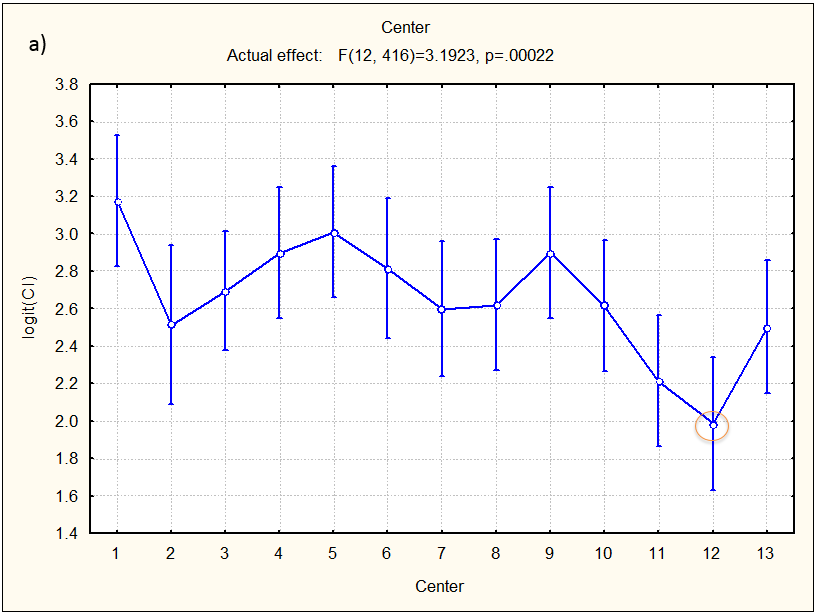
\includegraphics[width=.49\textwidth]{./cap3/YES_results_a.png}
%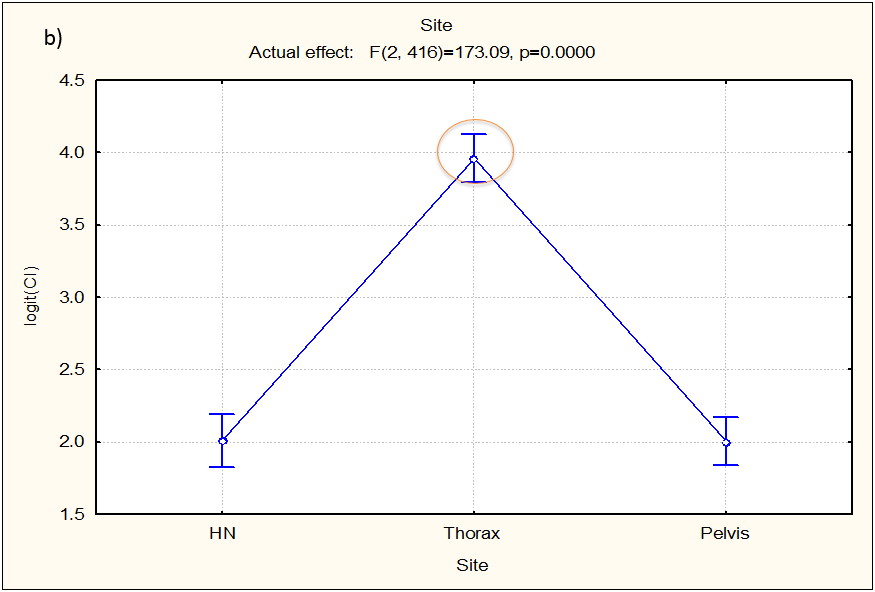
\includegraphics[width=.49\textwidth]{./cap3/YES_results_b.png}
%\caption{(a) risultati del confronto per quanto riguarda l'accuratezza globale delle deformazioni effettuate dai singoli centri. (b) risultati dell'accuratezza raggiunta considerando tutti i centri a seconda del sito di interesse. I valori statisticamente differenti dal campione sono cerchiati in rosso. Il test statistico utilizzato è del tipo ANOVA (\textit{ANalysis Of VAriances}).}
%\label{fig:YES_results}
%\end{figure}

Dal primo risultato si può evincere che i software commerciali esistenti portano a soluzioni di precisione comparabile pur implementando algoritmi differenti tra loro. Le performance relative al centro fuori fluttuazione statistica sono imputabili ad un differente livello di training degli operatori coinvolti piuttosto che ad un inferiorità dell'algoritmo utilizzato.

Il secondo risultato è spiegabile con la peculiarità del sito toracico (tumore polmonare) rispetto ai siti testa-collo e pelvico. In questi ultimi, molti dei tessuti coinvolti risultano essere differenti di pochi livelli nella scala di grigi (basso contrasto) per cui è necessario guidare la deformazione con varie ROI di controllo (il coefficiente di correlazione dei grigi non è sufficiente ad ottenere una deformazione accurata). Diversa è la situazione per il caso toracico in cui il tessuto tumorale all'interno del polmone risulta essere ad alto contrasto con il materiale circostante (aria) per cui la deformazione risulta semplice da trovare da parte dell'algoritmo, senza bisogno di particolari `aiuti'.\\

Oltre ai risultati ottenuti a livello multicentrico, il lavoro è stato approfondito nell'ambito di questa tesi con l'intento di sviluppare dei protocolli di registrazione deformabile sito-specifici propedeutici al commissioning del TPS RayStation per l'adaptive radiotherapy. 
%Alla data di redazione di questa tesi (Aprile 2016) l'ottimizzazione dei protocolli è ancora in via di sviluppo, presenteremo qui di seguito i risultati preliminari.

A questo proposito, durante la creazione delle deformazioni per lo studio multicentrico si è distinto l'approccio finalizzato a stressare l'algoritmo (orientato ad ottenere il miglior risultato possibile) da quello che può essere un approccio più orientato alla routine clinica. Più precisamente, dati uno studio CT di riferimento ed uno deformato, il metodo più preciso di effettuare una registrazione deformabile consiste nell'utilizzare una risoluzione di griglia molto fitta assieme all'impiego di numerose ROI di controllo che guidano l'algoritmo. Usualmente le ROI di controllo rappresentano degli organi a basso contrasto rispetto ai tessuti circostanti che l'algoritmo non riesce ad individuare con il solo termine di correlazione della Eq.\eqref{eq:def}. Volendo ad es. utilizzare la vescica come ROI di controllo in una deformazione del distretto pelvico, è necessario che questa sia delineata nello studio di riferimento e nello studio deformato. In un'implementazione di adaptive radiotherapy clinica con valutazione dosimetrica di ogni seduta di trattamento (approccio più preciso ed affidabile), l'utilizzo di una ROI di controllo per la registrazione deformabile presuppone la sua delineazione su ogni studio, operazione che può risultare estremamente time-consuming in un'ottica di routine clinica. Tipicamente il numero di sedute di trattamento di un paziente standard si aggira tra 20 e 30. Senza nessun ausilio le ROI di controllo andrebbero contornate su tutti gli studi CBCT acquisiti prima di ogni seduta di trattamento.

Per i motivi sopra citati, il principio fondante lo sviluppo dei protocolli di registrazione deformabile è stato quello di trovare il miglior compromesso tra precisione della deformazione ed impiego di ROI di controllo. Accanto a ciò sono in corso di studio anche i vari strumenti di contornazione semi-automatica offerti dal TPS RayStation per velocizzare la delineazione di ROI di controllo.

I protocolli risultano essere in via di perfezionamento in accordo con i risultati che emergeranno nelle successive fasi dello studio multicentrico. Verranno presentati nelle sezioni seguenti i risultati preliminari a cui si è giunti nelle fasi finali di questo lavoro di tesi. 

\subsection{Protocollo di registrazione deformabile - Torace}
Il cambiamento anatomico proposto dal gruppo multicentrico per il sito toracico consiste in una riduzione di volume di un tumore polmonare (vedi Fig.\ref{fig:YES_thorax}). 
\begin{figure}
\centering
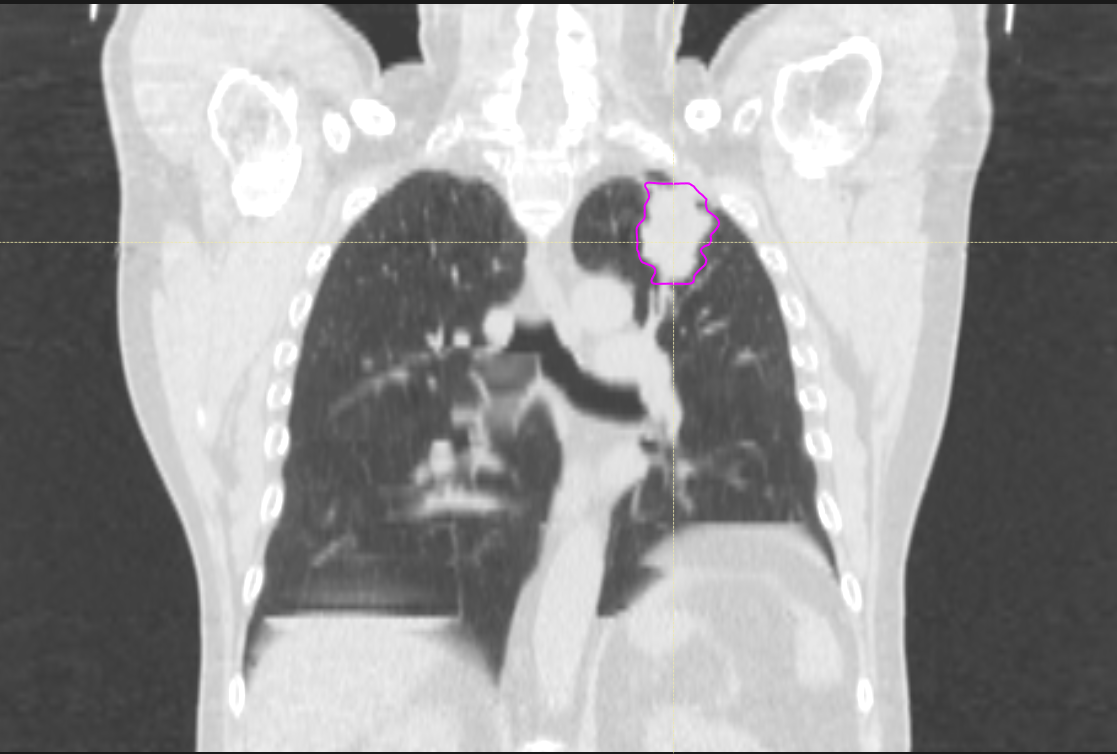
\includegraphics[width=.48\textwidth]{./cap3/YES_Thorax.png}
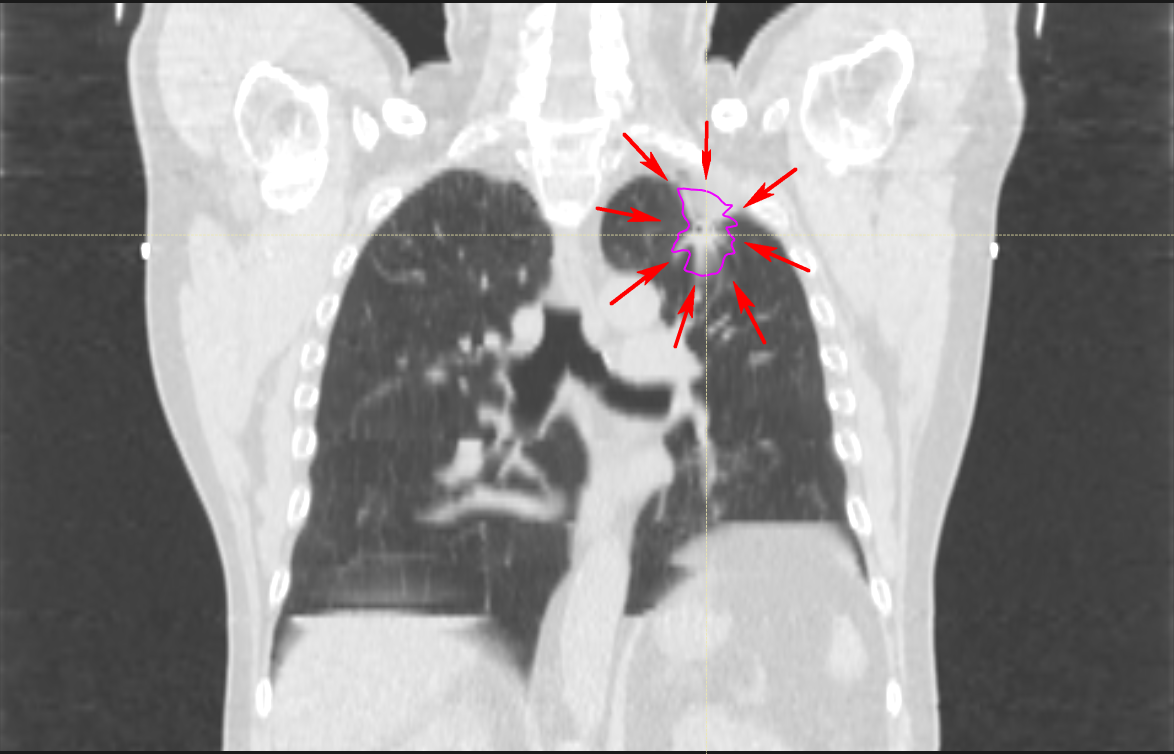
\includegraphics[width=.48\textwidth]{./cap3/YES_Thorax_shrink.png}
\caption{Studio multicentrico - sito toracico: riduzione di volume del tumore polmonare.}
\label{fig:YES_thorax}
\end{figure}
Il razionale dello sviluppo del protocollo di deformazione per questo sito si articola nei seguenti punti:
\begin{itemize}
\item La massa oggetto del cambiamento ha un alto contrasto con il tessuto circostante. Per questo motivo la deformazione da effettuare è semplice da trovare da parte dell'algoritmo senza ausilio di ROI di controllo (il solo termine di correlazione dei livelli di grigio è sufficiente a calcolare una deformazione accurata).
\item La zona di interesse da deformare riguarda una piccola porzione dell'intero studio CT. Per questo motivo ha senso ridurre la zona di analisi dell'algoritmo unicamente alla parte di interesse. \`E stato osservato che questa operazione aumenta sia la velocità di esecuzione che la precisione della deformazione finale. Lo strumento che RayStation offre in questo caso è detto \textit{Focus ROI}. Definita una \textit{Focus ROI}, il sistema applica l'algoritmo di deformazione unicamente all'interno di essa. 
\end{itemize}
Sulla base di queste considerazioni e dell'esperienza maturata, la proposta di protocollo per il sito toracico è la seguente:
\begin{enumerate}
\item Si effettua una registrazione rigida tra i due studi, privilegiando le strutture ossee.
\item Si effettua una registrazione deformabile senza ROI di controllo ma utilizzando come ROI di Focus il PTV espanso di 1 centimetro.
\end{enumerate}


\subsection{Protocollo di registrazione deformabile - Testa-Collo}
Nel caso del sito testa-collo la deformazione proposta corrisponde alla tipica riduzione del volume linfodonodale a livello delle parotidi (segno della risposta alla terapia, Fig.\ref{fig:YES_HN}). Questo cambiamento anatomico è di grande interesse per la radioterapia adattiva. Come illustrato nella Fig.\ref{fig:HN_DVH}, la riduzione del volume linfonodale comporta usualmente lo spostamento delle parotidi nella zona ad alta dose. L'ingresso di questi organi a rischio nella zona ad alta dose può portare ad un esito di radiotossicità che non è aspettato se si osserva unicamente il piano di trattamento iniziale.

\begin{figure}
\centering
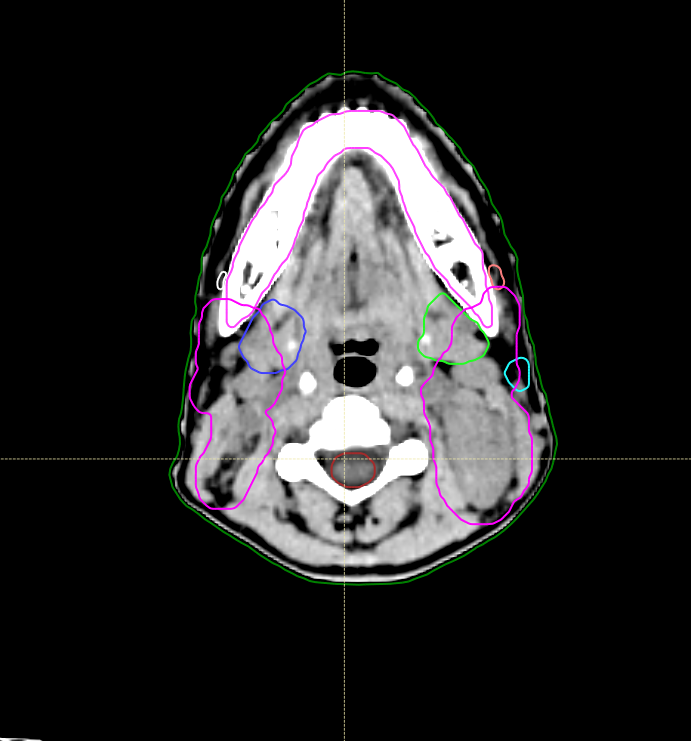
\includegraphics[width=.48\textwidth]{./cap3/YES_HN.png}
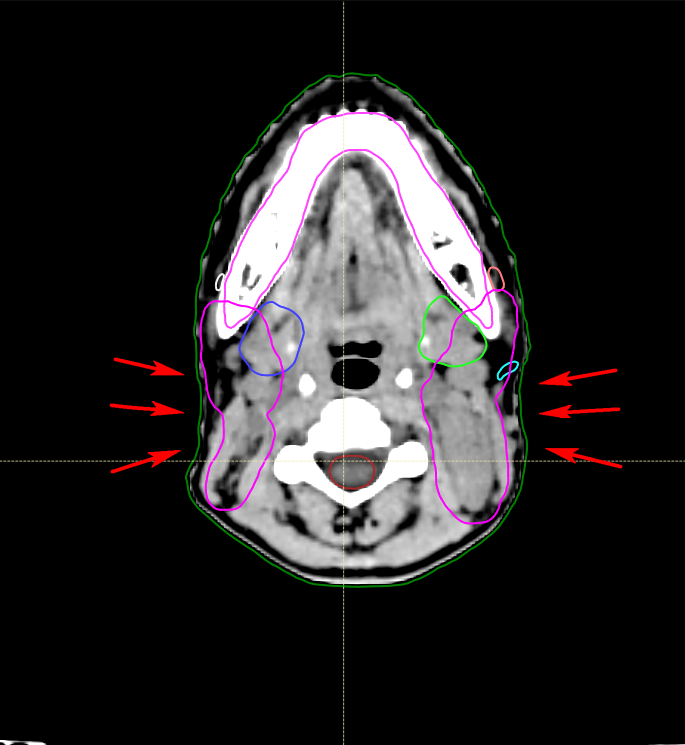
\includegraphics[width=.48\textwidth]{./cap3/YES_HN_shrink.png}
\caption{Studio multicentrico - caso testa-collo: riduzione del volume linfonodale.}
\label{fig:YES_HN}
\end{figure}

L'approccio che ha portato alla stesura del protocollo per le deformazioni del sito testa-collo è basato sui seguenti ragionamenti:
\begin{itemize}
\item Gli organi coinvolti in questo distretto sono pressoché stabili. Più precisamente, anche in presenza di deformazioni, i rapporti anatomici dei tessuti molli con i segmenti ossei sono usualmente conservati.
\item Il tipo di deformazione che si osserva è `prevedibile'. Più precismanete, ci si aspetta che nel corso del trattamento si va incontro ad una riduzione del volume linfonodale.
\end{itemize}
Sulla base di queste considerazioni la proposta di protocollo per il sito toracico è la seguente:
\begin{enumerate}
\item Si effettua una registrazione rigida tra i due studi, privilegiando le strutture ossee.
\item Si effettua una registrazione deformabile utilizzando come ROI di controllo la ROI che rappresenta il contorno del paziente (denominata \textit{External}). Questo perché il cambiamento anatomico è prevedibile e coinvolge maggiormente il contorno del paziente, lasciando le zone interne invariate. La delineazione di questa ROI di controllo è immediata qualora debba essere fatta su molteplici studi grazie agli strumenti di contornazione automatica messi a disposizione da RayStation. Con queste scelte, il protocollo risulta essere un buon compromesso tra precisione della deformazione (come dimostrato dal confronto con gli altri centri) e fattibilità a livello di routine clinica.
\end{enumerate}


\subsection{Protocollo di registrazione deformabile - Prostata}
Il cambiamento del riempimento degli organi interni al distretto pelvico (retto e vescica, Fig.\ref{fig:YES_PR}) rende questo sito uno dei più complessi da trattare con approccio di adaptive radiotherapy. 


Le considerazioni propedeutiche alla stesura del protocollo sono state le seguenti:
\begin{itemize}
\item Se nei casi torace e testa-collo i volumi di interesse si deformano con un andamento temporale prevedibile (monotono decrescente in caso di risposta alla terapia o monotono crescente in caso di non-risposta e progressione), i volumi nel distretto pelvico sono soggetti a variazioni casuali legate alla preparazione e alla compliance del paziente.
\item Come ulteriore difficoltà vi è il basso contrasto tra gli organi coinvolti nella deformazione. Ciò rende necessario l'utilizzo di ROI di controllo per guidare la deformazione.
\end{itemize}
 
Il protocollo proposto per questo sito consiste nei seguenti passaggi:
\begin{enumerate}
\item Si effettua una registrazione rigida tra i due studi, privilegiando le strutture ossee.
\item Si contornano sugli studi deformati le ROI corrispondenti agli organi vescica, retto e prostata con vescicole seminali. Queste ROI vengono utilizzate come ROI di controllo per guidare la deformazione nella zona a basso contrasto.
\end{enumerate}
L'applicazione clinica di questo protocollo può risultare molto time-consuming in quanto richiede un importante intervento dell'operatore nella contornazione delle ROI di controllo. Per ovviare a questo limite sono in studio a livello multicentrico le soluzioni di contornazione automatica offerte dal TPS.

\begin{figure}
\centering
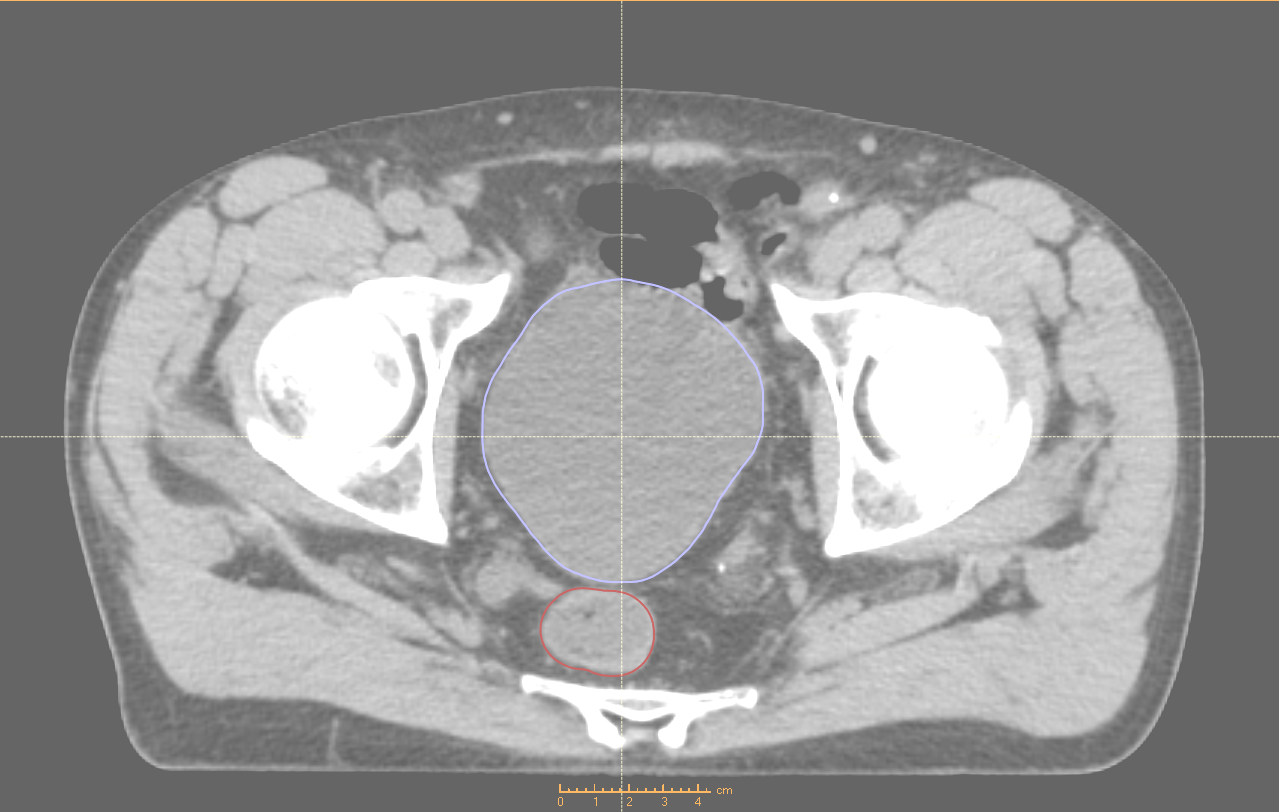
\includegraphics[width=.48\textwidth]{./cap3/YES_PR.png}
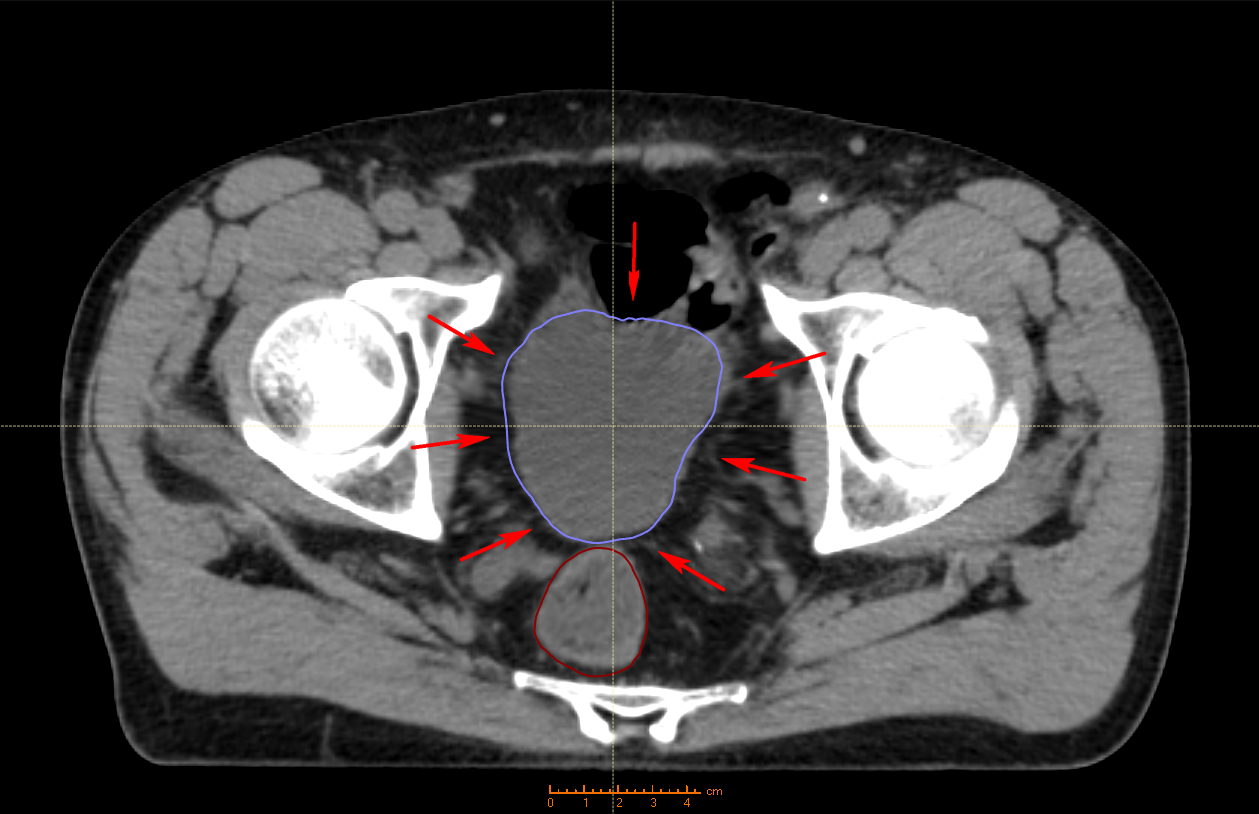
\includegraphics[width=.48\textwidth]{./cap3/YES_PR_shrink.png}
\caption{Studio multicentrico - caso prostata: riduzione del volume vescicale ed espansione del volume rettale.}
\label{fig:YES_PR}
\end{figure}


L'applicazione dei protocolli preliminari mostrati ha portato a deformazioni di precisione comparabile con gli altri centri. La discussione approfondita riguardo il confronto e l'eventuale ottimizzazione a livello multicentrico è programmata nelle prossime fasi dello studio.


\section{Studio multicentrico per predire la necessità di adattare il piano}
Lo studio multi-centrico cui si è presi parte fa parte di un progetto di ricerca del Ministero della Salute, dal titolo: \textit{``Dose warping methods for IGRT and Adaptive RT: dose accumulation based on organ motion and anatomical variations of the patients during radiation therapy treatments''}. Lo studio si pone come fine quello di sviluppare un metodo predittivo in grado di fornire parametri quantitativi che aiutino il medico radioterapista ed il fisico medico a decidere il momento in cui applicare o meno un processo di radioterapia adattiva sul determinato paziente.

Un approccio di tal genere appare quanto mai utile nelle realtà cliniche moderne in cui un processo di radioterapia adattiva è inapplicabile su larga scala a tutta la popolazione di pazienti a causa dei sottoprocessi time consuming da mettere in campo per questo scopo (primo tra tutti l'identificazione giornaliera dei volumi di interesse per il trattamento che dovrebbe essere eseguita dal medico radioterapista). Questa considerazione è supportata anche da evidenze in letteratura \cite{Capelle2012} secondo cui un approccio di radioterapia adattiva su pazienti non accuratamente selezionati porta a benefici clinici trascurabili ed ad un impiego improprio di risorse.


La patologia su cui si è inizialmente focalizzato lo studio è quella dei tumori riguardanti il distretto testa-collo. La prima fase dello studio è stata quella di caratterizzare il comportamento dei pazienti affetti da questa patologia tramite un'analisi retrospettiva del database posseduto dal centro coordinatore (Policlinico di Modena). \`E stata analizzata una coorte di 40 pazienti. In accordo con il comportamento generale, la variazione più importante che si registra durante il corso del trattamento radioterapico è la riduzione del volume delle parotidi dovuta a fenomeni di risposta alla terapia e ad un generale dimagrimento del paziente. % (Fig.\ref{fig:Modena_DV}).
%\begin{figure}
%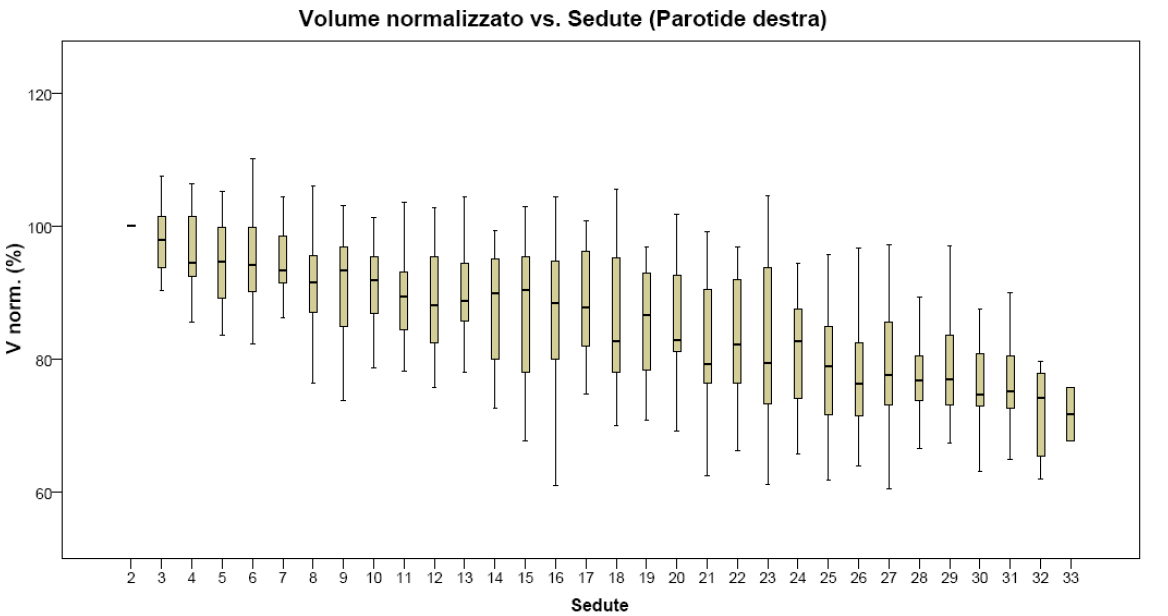
\includegraphics[width=.8\textwidth]{./cap3/Modena_volDecrease.png}\\
%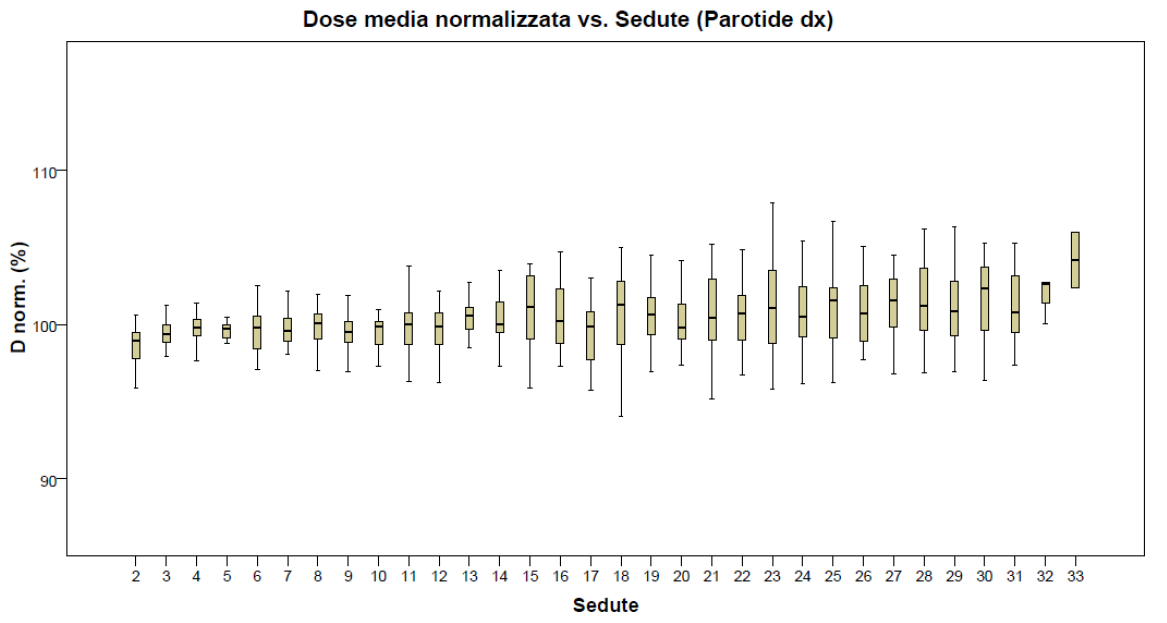
\includegraphics[width=.8\textwidth]{./cap3/Modena_dosIncrease.png}
%\caption{(a) trend di decrescita del volume della parotide destra e conseguente trend di incremento (b) della dose media.}
%\label{fig:Modena_DV}
%\end{figure}

L'analisi retrospettiva è stata ulteriormente approfondita correlando le variazioni di dose e di volume sotto forma di scatter plot come in Fig.\ref{fig:Modena_trend}. Quello che si può osservare è una divisione della popolazione in due sottogruppi: il gruppo di pazienti che subisce grandi variazioni dosimetriche e volumetriche (che potrebbero beneficiare di un approccio adattivo) ed il gruppo di pazienti che invece rimane entro un limitato range di variabilità rispetto alle condizioni iniziali.

\begin{figure}
\centerline{
\hspace{-1.6cm}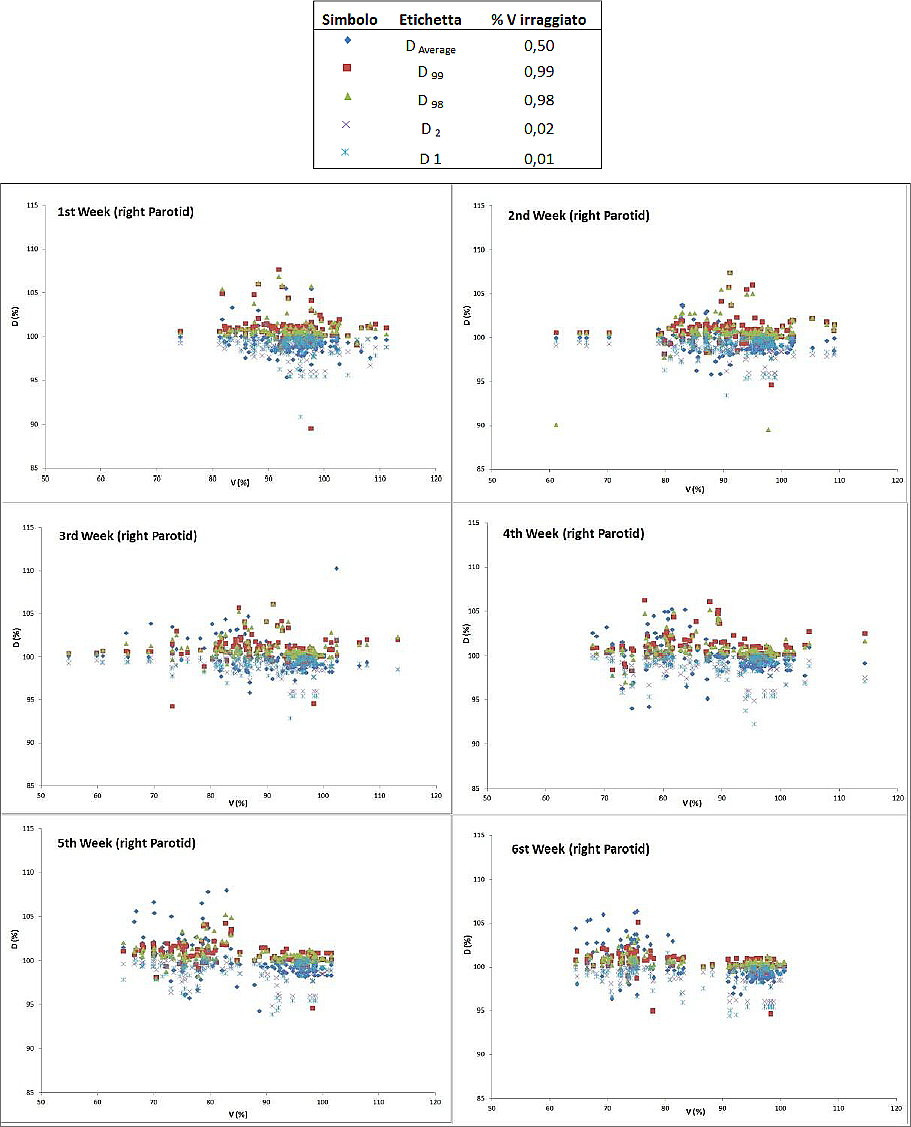
\includegraphics[width=1.32\textwidth]{./cap3/Modena_trend_s.png}}
\caption{Analisi scatter plot delle sei settimane di trattamento per la parotide destra. Tutte le variazioni sono normalizzate rispetto al valore iniziale di dose o di volume per omogeneizzare il campione (i.e. un punto vicino alla coordinata (100,100) rappresenta una variazione volumetrica e dosimetrica nulla rispetto alla condizione iniziale).}
\label{fig:Modena_trend}
\end{figure}

Sulla base di queste di queste osservazioni il centro coordinatore ha sviluppato un algoritmo capace di effettuare una separazione statistica (\textit{clustering}) delle due popolazioni in modo da individuare i pazienti che possono beneficiare di un approccio adattivo nonché la settimana per cui la differenza tra le popolazioni diventa significativa (ipotetica settimana in cui si può pensare di effettuare una modifica adattiva del piano)\cite{Guidi2015} (Fig.\ref{fig:Modena_cluster}). Le soglie di variazione che stabiliscono la separazione dei due cluster sono:
\begin{itemize}
\item Variazione del volume dell'organo rispetto al volume iniziale di più del 30\%.
\item Variazione di dose all'interno dell'organo maggiori del 10\%.
\end{itemize}
\begin{figure}
\centering
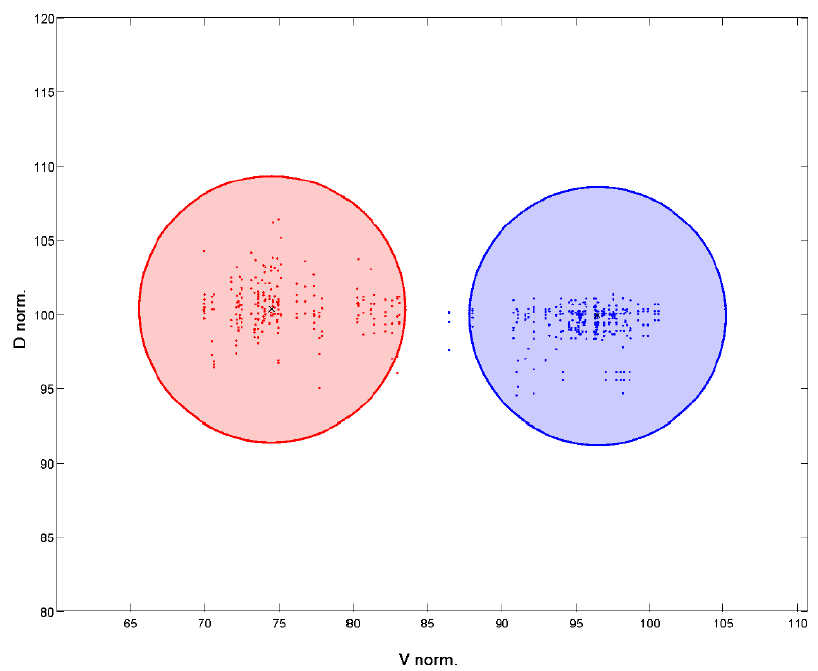
\includegraphics[width=.7\textwidth]{./cap3/Modena_cluster.png}
\caption{Esempio di clusterizzazione dei dati per la parotide valutata nell'ultima settimana di trattamento per una coorte di 40 pazienti. In blu: pazienti con variazioni volumetriche e dosimetriche non eccessive per cui non è necessario un re-planning. In rosso: pazienti con variazioni volumetriche e dosimetriche ampie per cui è consigliato un re-planning.}
\label{fig:Modena_cluster}
\end{figure}

Lo studio multi-centrico ha coinvolto quattro centri italiani tra cui la ASL di Teramo. Ogni centro aveva il compito di reclutare una serie di pazienti con neoplasia del distretto testa-collo di cui sono state osservate variazioni significative durante il corso del trattamento e di inviarle al centro coordinatore. I trattamenti presi in considerazione hanno durata di circa sei settimane. I pazienti di ogni centro sono stati analizzati dal centro coordinatore ed è stato ricavato l'outcome predetto dall'algoritmo. \\
I risultati sono riportati in Fig.\ref{fig:Modena_results}a. Dai grafici mostrati si può desumere che la percentuale di pazienti che beneficerebbe di una ripianificazione adattiva aumenta con il proseguire del trattamento. Questo trend è stato osservato per tutti i centri coinvolti. In particolare si nota che l'inversione tra la percentuale di pazienti che non necessitano di ripianificazione e quelli per cui una ripianificazione è suggerita avviene durante la quarta settimana di trattamento. Questa evidenza si riscontra con più precisione osservando il comportamento della popolazione ottenuto mediando i risultati dei singoli centri (Fig.\ref{fig:Modena_results}b).

\begin{figure}
\centering
a)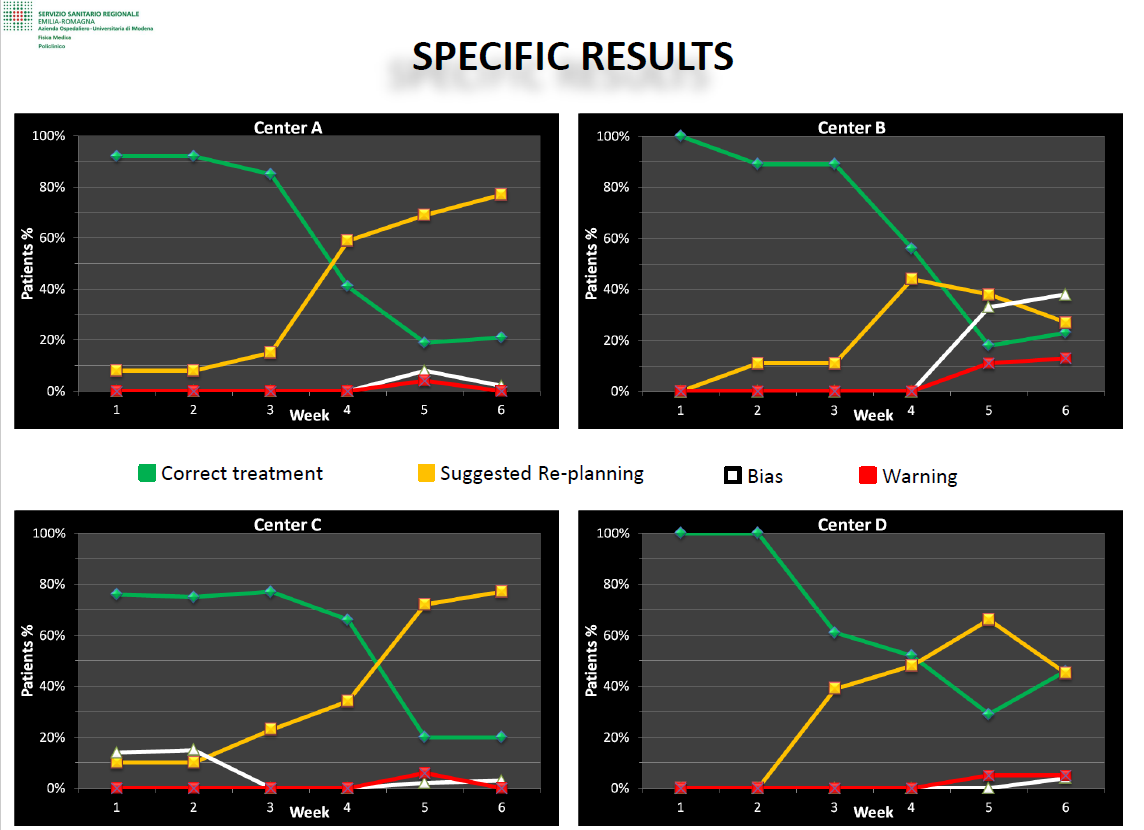
\includegraphics[width=.95\textwidth]{./cap3/Modena_specRes.png}\\
b)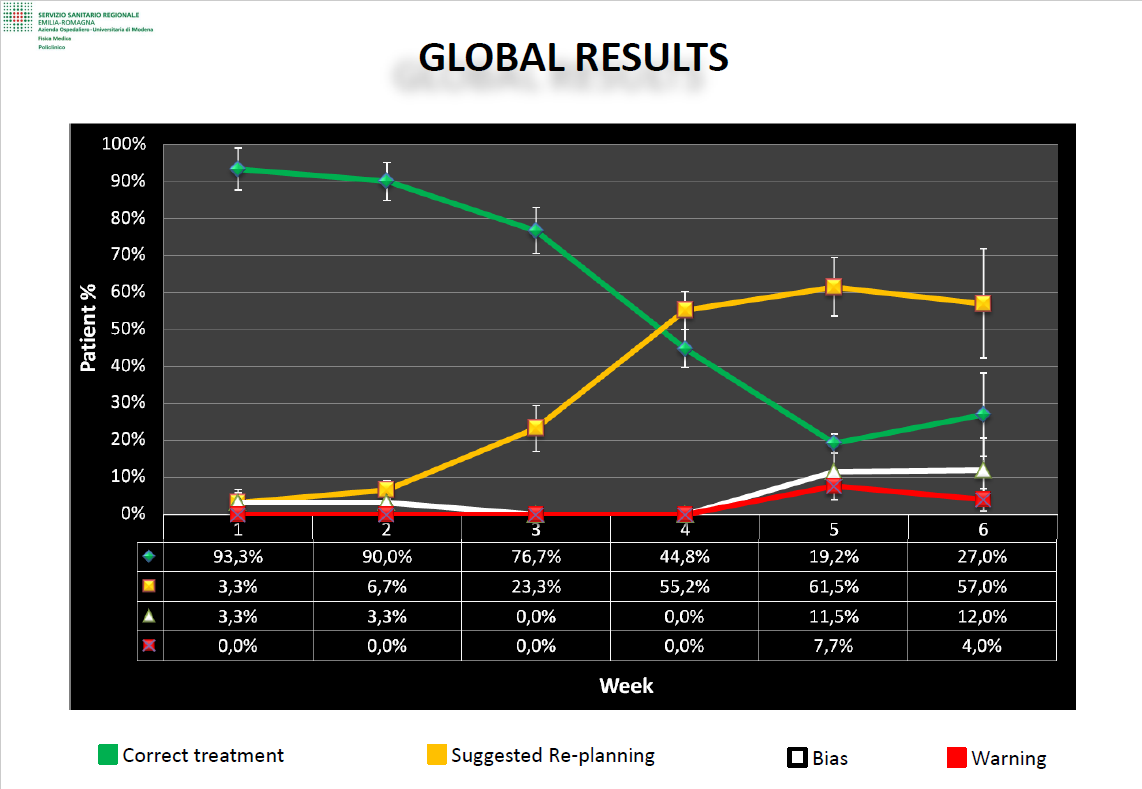
\includegraphics[width=.95\textwidth]{./cap3/Modena_globRes.png}
\caption{Risultati dell'analisi multicentrica per la predizione del tempo ottimale di ripianificazione distinti per centro (a) e mediati su tutti i centri (b). \textit{Correct treatment:} percentuale di pazienti che non necessitano di ripianificazione; \textit{Suggested Re-planning:} percentuale di pazienti per cui è suggerita una ripianficazione; \textit{Bias:} percentuale di pazienti per cui l'algoritmo non è stato in grado di discriminare il trend; \textit{Warning:} percentuale di pazienti per cui si sono rilevate alte variabilità fuori dai limiti di applicabilità dell'algoritmo (possibile errore di set-up del paziente).}
\label{fig:Modena_results}
\end{figure}

A seguito dei risultati ottenuti in questo studio, è in corso di svolgimento la redazione di un protocollo di radioterapia adattiva locale secondo il quale si prevede una valutazione multidisciplinare dei pazienti testa-collo all'inizio della quarta settimana di trattamento per decidere o meno un adattamento del piano sulla base della particolare situazione clinica. 

